\documentclass[tikz,border=18pt]{standalone}
\usepackage[T1]{fontenc}
\usepackage{lmodern}
\usetikzlibrary{arrows.meta,backgrounds}
\hyphenpenalty=10000

\definecolor{ink}{HTML}{24314A}
\definecolor{muted}{HTML}{667085}
\definecolor{blue}{HTML}{6485F7}
\definecolor{bluefill}{HTML}{EEF3FF}
\definecolor{pink}{HTML}{DF78AD}
\definecolor{pinkfill}{HTML}{FFF0F7}
\definecolor{purple}{HTML}{8B6DE0}
\definecolor{purplefill}{HTML}{F4F0FF}
\definecolor{green}{HTML}{31987D}
\definecolor{greenfill}{HTML}{EAF9F4}

\tikzset{
  stage/.style={
    rounded corners=4pt,
    very thick,
    align=center,
    minimum height=18mm,
    text width=34mm,
    inner sep=4pt,
    font=\sffamily\small,
    text=ink
  },
  host/.style={stage,draw=blue,fill=bluefill},
  server/.style={stage,draw=purple,fill=purplefill},
  widget/.style={stage,draw=pink,fill=pinkfill},
  result/.style={stage,draw=green,fill=greenfill},
  forward/.style={-{Latex[length=3mm,width=2mm]},line width=1.15pt,draw=ink!68},
  return/.style={-{Latex[length=3mm,width=2mm]},line width=1.2pt,draw=green,dashed},
  laneTitle/.style={font=\sffamily\bfseries\small,text=ink},
  footer/.style={font=\sffamily\scriptsize,text=muted,align=center}
}

\begin{document}
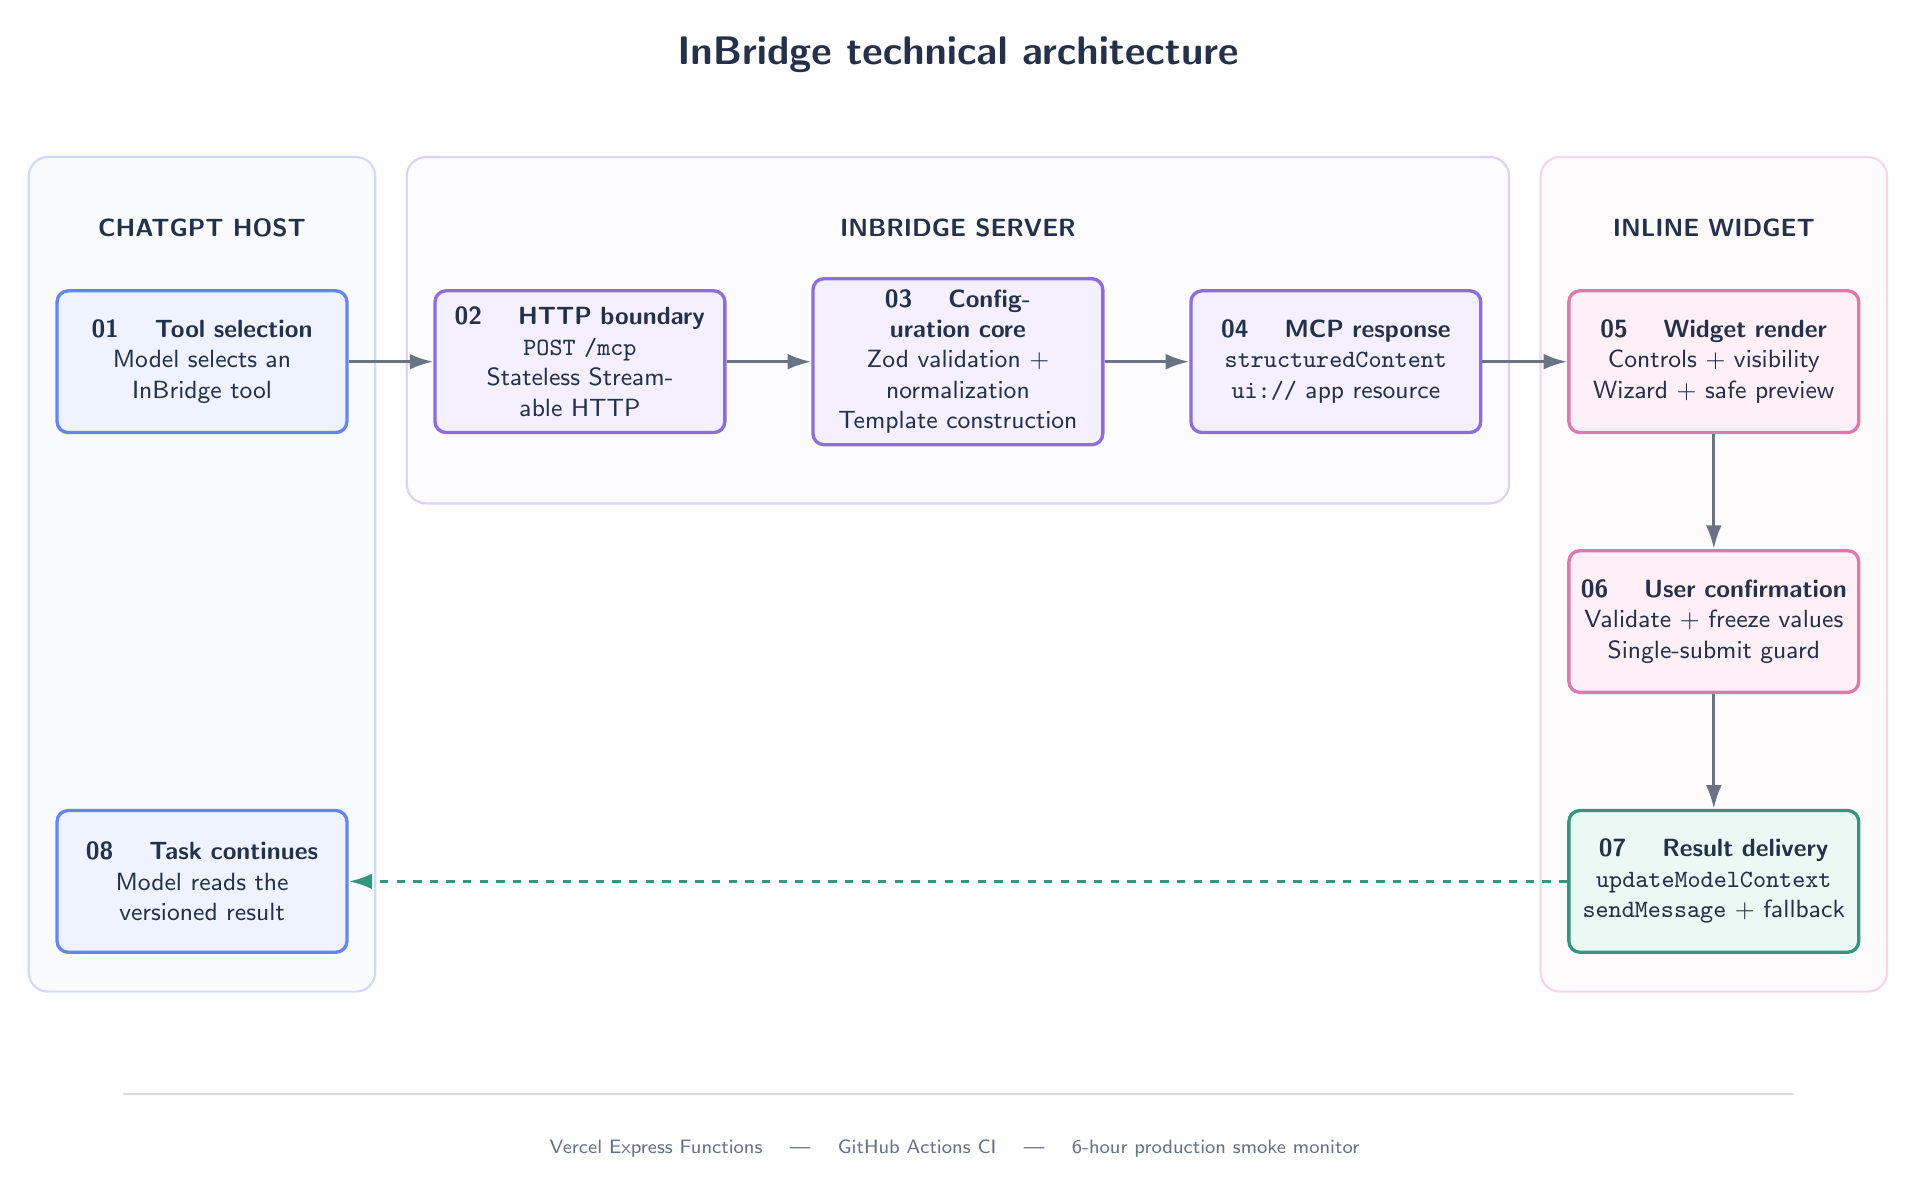
\begin{tikzpicture}[x=1mm,y=1mm]
  % Fixed ownership regions keep the main flow horizontal and the return path isolated.
  \begin{scope}[on background layer]
    \path[draw=blue!30,fill=blue!3,rounded corners=7pt,line width=.8pt]
      (-22,2) rectangle (22,-104);
    \path[draw=purple!30,fill=purple!3,rounded corners=7pt,line width=.8pt]
      (26,2) rectangle (166,-42);
    \path[draw=pink!30,fill=pink!3,rounded corners=7pt,line width=.8pt]
      (170,2) rectangle (214,-104);
  \end{scope}

  \node[laneTitle] at (0,-7) {CHATGPT HOST};
  \node[laneTitle] at (96,-7) {INBRIDGE SERVER};
  \node[laneTitle] at (192,-7) {INLINE WIDGET};

  \node[host] (tool) at (0,-24) {
    \textbf{01 \quad Tool selection}\\
    Model selects an InBridge tool
  };
  \node[server] (http) at (48,-24) {
    \textbf{02 \quad HTTP boundary}\\
    \texttt{POST /mcp}\\
    Stateless Streamable HTTP
  };
  \node[server] (core) at (96,-24) {
    \textbf{03 \quad Configuration core}\\
    Zod validation + normalization\\
    Template construction
  };
  \node[server] (response) at (144,-24) {
    \textbf{04 \quad MCP response}\\
    \texttt{structuredContent}\\
    \texttt{ui://} app resource
  };

  \node[widget] (render) at (192,-24) {
    \textbf{05 \quad Widget render}\\
    Controls + visibility\\
    Wizard + safe preview
  };
  \node[widget] (confirm) at (192,-57) {
    \textbf{06 \quad User confirmation}\\
    Validate + freeze values\\
    Single-submit guard
  };

  \node[result] (delivery) at (192,-90) {
    \textbf{07 \quad Result delivery}\\
    \texttt{updateModelContext}\\
    \texttt{sendMessage} + fallback
  };
  \node[host] (continue) at (0,-90) {
    \textbf{08 \quad Task continues}\\
    Model reads the versioned result
  };

  \draw[forward] (tool.east) -- (http.west);
  \draw[forward] (http.east) -- (core.west);
  \draw[forward] (core.east) -- (response.west);
  \draw[forward] (response.east) -- (render.west);
  \draw[forward] (render.south) -- (confirm.north);
  \draw[forward] (confirm.south) -- (delivery.north);
  \draw[return] (delivery.west) -- (continue.east);

  \node[font=\sffamily\bfseries\Large,text=ink] at (96,15)
    {InBridge technical architecture};
  \node[footer] at (96,-124) {
    Vercel Express Functions \quad | \quad GitHub Actions CI
    \quad | \quad 6-hour production smoke monitor
  };
  \draw[draw=ink!18,line width=.8pt] (-10,-117) -- (202,-117);
\end{tikzpicture}
\end{document}
